Next step was to do the analysis on the smaller scale and see if sentiment changes between tweets collected 3 days prior and post-release. Results are shown in Table \ref{table:BeforeAfterReleaseSentiment}.

\begin{table}[H]
\centering
\begin{tabular}{ |p{3cm}|p{3cm}|p{3cm}|}
 \hline
\textbf{Project }& \textbf{Before}& \textbf{After}\\
 \hline
 NodeJS   & 0.707 & 0.709\\ \hline
 EmberJS   & 0.719 & 0.719\\ \hline
 VueJS   & 0.694 & 0.708\\ \hline 
 Symfony & 0.73 & 0.729\\ \hline   
 AngularJS   & 0.718 & 0.719\\ \hline
 CakePhp & 0.71 & 0.702\\ \hline 
 Bower   & 0.634 & 0.638\\ \hline 
 Laravel & 0.683 & 0.696\\ \hline
 Gulp & 0.608 & 0.573\\ \hline
 Yii & 0.643 & 0.606\\ \hline
 Bootstrap & 0.713 & 0.693\\ \hline
\end{tabular}
\caption{Average sentiment of tweets 3 days before and after releases}
\label{table:BeforeAfterReleaseSentiment}
\end{table}

From the data shown in table is visible, that there is no big sentiment shift caused by releases on the small time frame. The biggest noticable pattern (nicely displayed in Figure \ref{fig:sentimentChangeBeforeAfter}) is 4\% decrease in sentiment of seldom releasing projects. In groups which release often or normally, sentiment change was very small.

\begin{figure}[H]%
    \centering
	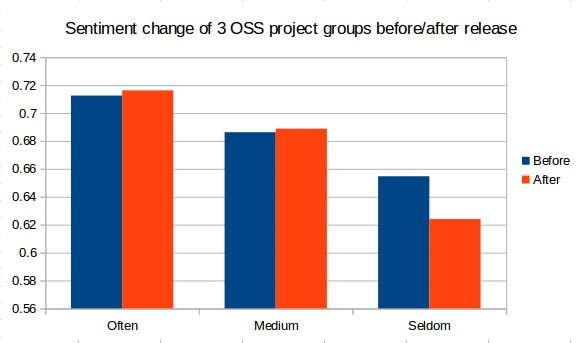
\includegraphics[width=10cm]{sentimentChangeBeforeAfter.jpg}
    \caption{Change in sentiment for all 3 OSS groups before/after release}%
    \label{fig:sentimentChangeBeforeAfter}%
\end{figure}

A clear pattern to notice in both figures (\ref{fig:weeklyAverageBarchart} and \ref{fig:sentimentChangeBeforeAfter}) is, that more often projects release, better their sentiment gets.